\documentclass{beamer}
\usepackage{amsmath,amsbsy,amsopn,amstext,amsfonts,amssymb}
\usepackage{isomath}
\usepackage{ulem}
%\linespread{1.6}  % double spaces lines
\usepackage{graphicx}
\usepackage{subfigure}
\usepackage{color}
\usepackage{optidef}  % define optimization problems
\usepackage{multicol}  % multiple columns
\usepackage{listings} % for python code
\usepackage{mathrsfs}

\usepackage{polynom}
\newcommand{\adj}{\mathrm{adj}}
\newcommand{\constrainedmin}[3]{
		\begin{mini*}|s|
		{#2}{#1}{}{}
		\addConstraint{#3}
		\end{mini*}
}

\newcommand{\rwbcomment}[1]{{\color{blue}RWB:#1}}
\newcommand{\defeq}{\stackrel{\triangle}{=}}
\newcommand{\abs}[1]{\left|#1\right|}
\newcommand{\norm}[1]{\left\|#1\right\|}
\newcommand{\iprod}[1]{\left<#1\right>}
\newcommand{\ellbf}{\boldsymbol{\ell}}
\newcommand{\nubf}{\boldsymbol{\nu}}
\newcommand{\mubf}{\boldsymbol{\mu}}
\newcommand{\abf}{\mathbf{a}}
\newcommand{\bbf}{\mathbf{b}}
\newcommand{\cbf}{\mathbf{c}}
\newcommand{\dbf}{\mathbf{d}}
\newcommand{\ebf}{\mathbf{e}}
\newcommand{\fbf}{\mathbf{f}}
\newcommand{\gbf}{\mathbf{g}}
\newcommand{\hbf}{\mathbf{h}}
\newcommand{\ibf}{\mathbf{i}}
\newcommand{\jbf}{\mathbf{j}}
\newcommand{\kbf}{\mathbf{k}}
\newcommand{\lbf}{\mathbf{l}}
\newcommand{\mbf}{\mathbf{m}}
\newcommand{\nbf}{\mathbf{n}}
\newcommand{\obf}{\mathbf{o}}
\newcommand{\pbf}{\mathbf{p}}
\newcommand{\qbf}{\mathbf{q}}
\newcommand{\rbf}{\mathbf{r}}
\newcommand{\sbf}{\mathbf{s}}
\newcommand{\tbf}{\mathbf{t}}
\newcommand{\ubf}{\mathbf{u}}
\newcommand{\vbf}{\mathbf{v}}
\newcommand{\wbf}{\mathbf{w}}
\newcommand{\xbf}{\mathbf{x}}
\newcommand{\ybf}{\mathbf{y}}
\newcommand{\zbf}{\mathbf{z}}
\newcommand{\Jbf}{\mathbf{J}}
\newcommand{\Acal}{\mathcal{A}}
\newcommand{\Bcal}{\mathcal{B}}
\newcommand{\Lcal}{\mathcal{L}}
\newcommand{\Ncal}{\mathcal{N}}
\newcommand{\Rcal}{\mathcal{R}}
\definecolor{darkolivegreen}{rgb}{0.33, 0.42, 0.18}

\makeatletter
\newenvironment<>{proofstart}[1][\proofname]{%
    \par
    \def\insertproofname{#1\@addpunct{.}}%
    \usebeamertemplate{proof begin}#2}
  {\usebeamertemplate{proof end}}
\newenvironment<>{proofcont}{%
  \setbeamertemplate{proof begin}{\begin{block}{}}
    \par
    \usebeamertemplate{proof begin}}
  {\usebeamertemplate{proof end}}
\newenvironment<>{proofend}{%
    \par
    \pushQED{\qed}
    \setbeamertemplate{proof begin}{\begin{block}{}}
    \usebeamertemplate{proof begin}}
  {\popQED\usebeamertemplate{proof end}}
\makeatother

\title{ECEn 671: Mathematics of Signals and Systems}
\author{Randal W. Beard}
\institute{Brigham Young University}
\date{\today}

\begin{document}

%-------------------------------
\begin{frame}
	\titlepage
\end{frame}


%%%%%%%%%%%%%%%%%%%%%%%%%%%%%%%%%%%%%%%%%%%%%%%%%%%%%%%%%%%%%%%%%
\section{Pseudo Inverse and the SVD}
\frame{\sectionpage}

%----------------------------------
\begin{frame}\frametitle{Pseudo Inverses of $A$}
	Least squares solution to $Ax=b$ (i.e. $\min\norm{Ax-b}_2$) where $A$-tall is
	\[ 
		\hat{x} = (A^H A)^{-1} A^H b \defeq A^\dagger b.
	\]
	
	\vfill
	
	Minimum norm solution to $Ax = b$ (i.e. $\min\norm{x}$ for $Ax=b$) where $A$-fat is
	\[
		x = A^H (A A^H)^{-1} b \defeq A^\dagger b. 
	\]
	
	\vfill
	
	How does the SVD help compute the pseudo inverse.  We will consider both when $A$ is full rank, and when $A$ is not full rank.
\end{frame}

%----------------------------------
\begin{frame}\frametitle{SVD and Least Squared: Full Rank $A$}
	Assume $A\in\mathbb{C}^{m\times n}$ is tall, i.e.,  $m > n$, and that 
	$\text{rank}(A) = n$.  Then
	\[
		A = 
			\begin{pmatrix}
				U_1 & U_2	
			\end{pmatrix}
			\begin{pmatrix}
				\Sigma \\ 0	
			\end{pmatrix}
			V^H
		= U_1 \Sigma V^H
	\]
	where $U_1\in\mathbb{C}^{m\times n}$, $\Sigma \in \mathbb{R}^{n\times n}$, and $V\in\mathbb{C}^{n\times n}$.
	
	\vfill
	
	Then
	\begin{align*}
		(A^HA)^{-1}A^H 
			&= (V\Sigma U_1^HU_1\Sigma V^H)^{-1}V\Sigma U_1^H\\
			&= (V\Sigma^2V^H)^{-1}V\Sigma U_1^H\\
			&= V\Sigma^{-2}V^HV\Sigma U_1^H\\
			&= V\Sigma^{-1}U_1^H
	\end{align*}
	where $\Sigma^{-1} = \text{diag}(\frac{1}{\sigma_1}, \dots, \frac{1}{\sigma_n})$.	
\end{frame}

%----------------------------------
\begin{frame}\frametitle{SVD and min Norm: Full Rank $A$}
	Assume $A\in\mathbb{C}^{m\times n}$ is fat, i.e.,  $m < n$, and that $\text{rank}(A) = m$.  Then
	\begin{align*}
		A &= U \begin{pmatrix}
		      		\Sigma & 0
		    	\end{pmatrix}
		    	\begin{pmatrix}
		  			V_1^H\\
		  			V_2^H
				\end{pmatrix} \\ 
		&= U\Sigma V_1^H				
	\end{align*}
	where $U\in\mathbb{C}^{m\times m}$, 
	$\Sigma=\text{diag}(\sigma_1, \dots, \sigma_m)$, 
	$V_1 \in \mathbb{C}^{n\times m}$.
	
	\vfill
	
	Then 
	\begin{align*}
		A^H (A A^H)^{-1} 
			&= V_1 \Sigma U^H(U\Sigma V_1^HV_1\Sigma U^H)^{-1}\\
			&= V_1 \Sigma U^H(U\Sigma^2U^H)^{-1}\\
			&= V_1 \Sigma U^HU\Sigma^{-2}U^H\\
			&= V_1 \Sigma^{-1}U^H
	\end{align*}
	where $\Sigma^{-1} = \text{diag}(\frac{1}{\sigma_1}, \dots, \frac{1}{\sigma_m})$
\end{frame}

%----------------------------------
\begin{frame}\frametitle{SVD and Pseudo Inverse: Not Full Rank $A$}
	Assume $A\in\mathbb{C}^{m\times n}$ and that $\text{rank}(A) = p < \min(m,n)$.  Then
	\[ 
		A = 
			\begin{pmatrix} 
				U_1 & U_2	
			\end{pmatrix}
			\begin{pmatrix}
				\Sigma & 0 \\ 0 & 0	
			\end{pmatrix}
			\begin{pmatrix}
				V_1^H \\ V_2^H	
			\end{pmatrix}
		= U_1 \Sigma V_1^H
	\]
	where
	$U_1\in\mathbb{C}^{m\times p}$, 
	$\Sigma = \text{diag}(\sigma_1, \dots, \sigma_p) \in \mathbb{R}^{p\times p}$,
	$V_1 \in \mathbb{C}^{n \times p}$.

	Consider the least squares problem
	\begin{align*}
		\hat{x} &= (A^HA)^{-1}A^Hb\\
		&= (V_1\Sigma_1U_1^HU_1\Sigma_1V_1^H)^{-1}V_1\Sigma_1U_1^Hb\\
		&= (V_1\Sigma_1^2V_1^H)^{-1}V_1\Sigma_1U_1^Hb\\
		&= V_1\Sigma_1^{-2}V_1^HV_1\Sigma_1U_1^Hb\\
		&= V_1\Sigma_1^{-1}U_1^Hb
	\end{align*}
	where 
	$\Sigma_1 = \text{diag}(\frac{1}{\sigma_1}, \dots, \frac{1}{\sigma_p})$.
\end{frame}

%----------------------------------
\begin{frame}\frametitle{SVD and Pseudo Inverse: Not Full Rank $A$}
	So we can compute it, but what did we do?  How do we interpret the solution since the inverse of $A^HA$ does not exist?
	
	\begin{center}
		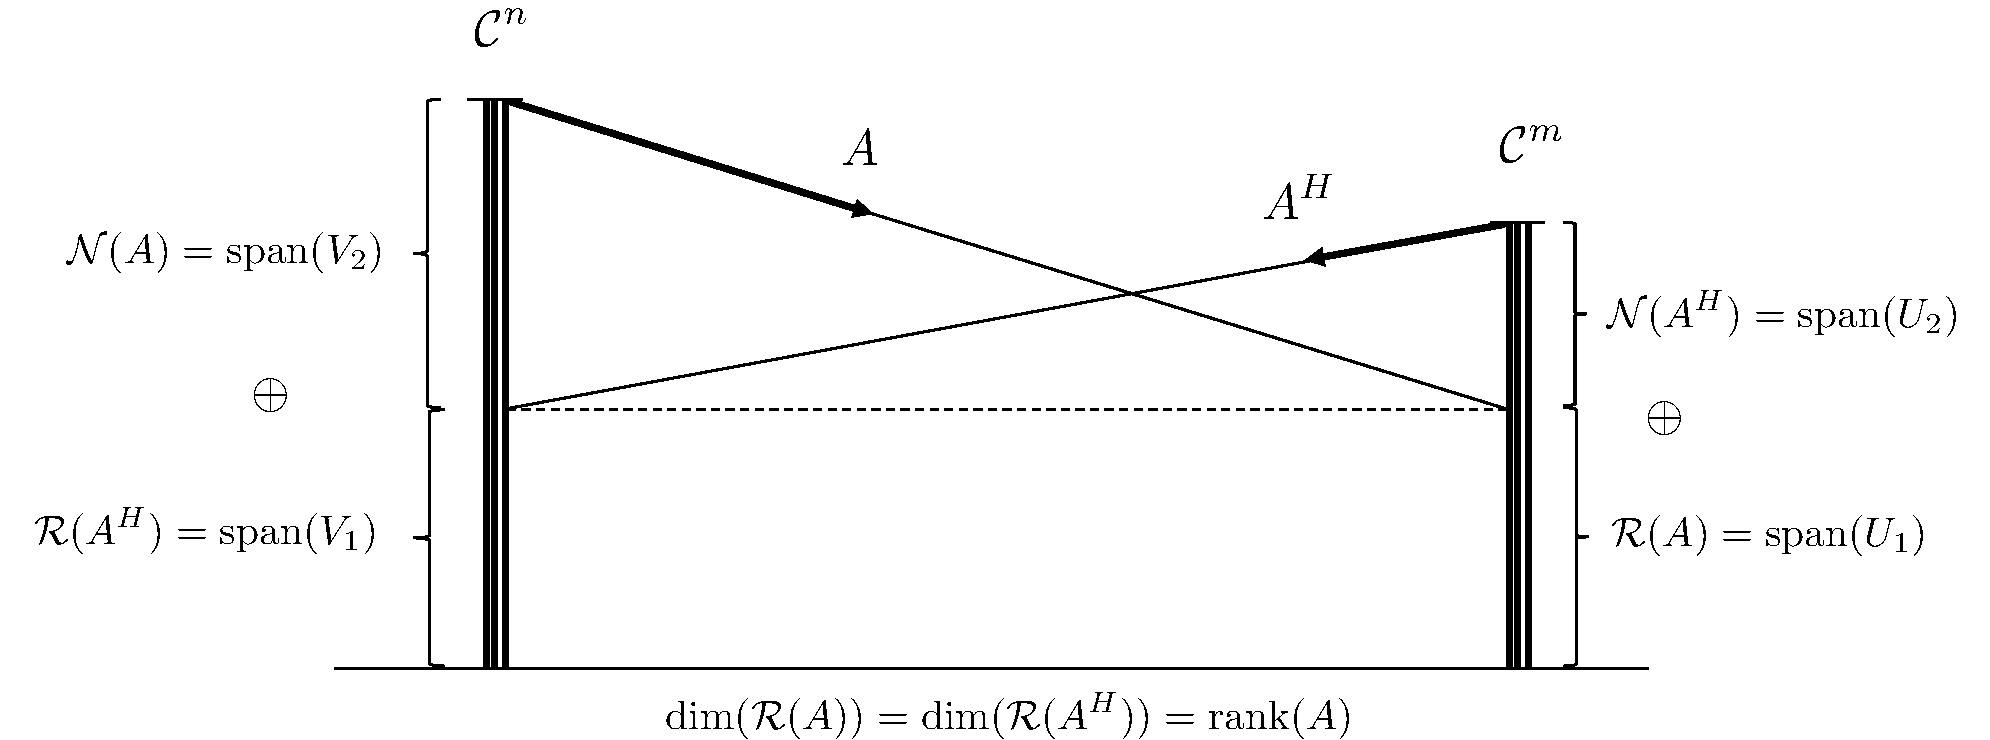
\includegraphics[width=0.9\textwidth]
			{figures/chap7_fundamental_subspace_3}
	\end{center}
	
	
	Find a solution to $Ax = b$ where $b \in \mathcal{R}(A)$.  But $\mathcal{N}(A)\neq \{0\}$ implies that there are more than one solution.
	
	\vfill
	
	Therefore, find the minimum norm $x$ that minimizes 
	$\norm{Ax - b}_2$.
\end{frame}

%----------------------------------
\begin{frame}\frametitle{SVD and Pseudo Inverse: Not Full Rank $A$}
	Note the following:
	\[ 
		\underbrace{U_1}_{m \times p}: \mathbb{C}^p \to \mathcal{R}(A) \subset \mathbb{C}^m
	\]
	so that
	\[ 
		U_1^\ast = U_1^H:\mathbb{C}^m\to\mathbb{C}^p.
	\]
	
	Also,
	\[ 
		\underbrace{V_1}_{n\times p}: \mathbb{C}^p \to 
			\mathcal{R}(A^H) \subset \mathbb{C}^n 
	\]
	so that
	\[ 
		V_1^H : \mathbb{C}^n \to \mathbb{C}^p.
	\]	
\end{frame}

%----------------------------------
\begin{frame}\frametitle{SVD and Pseudo Inverse: Not Full Rank $A$}
	So we have the following:
	\begin{center}
		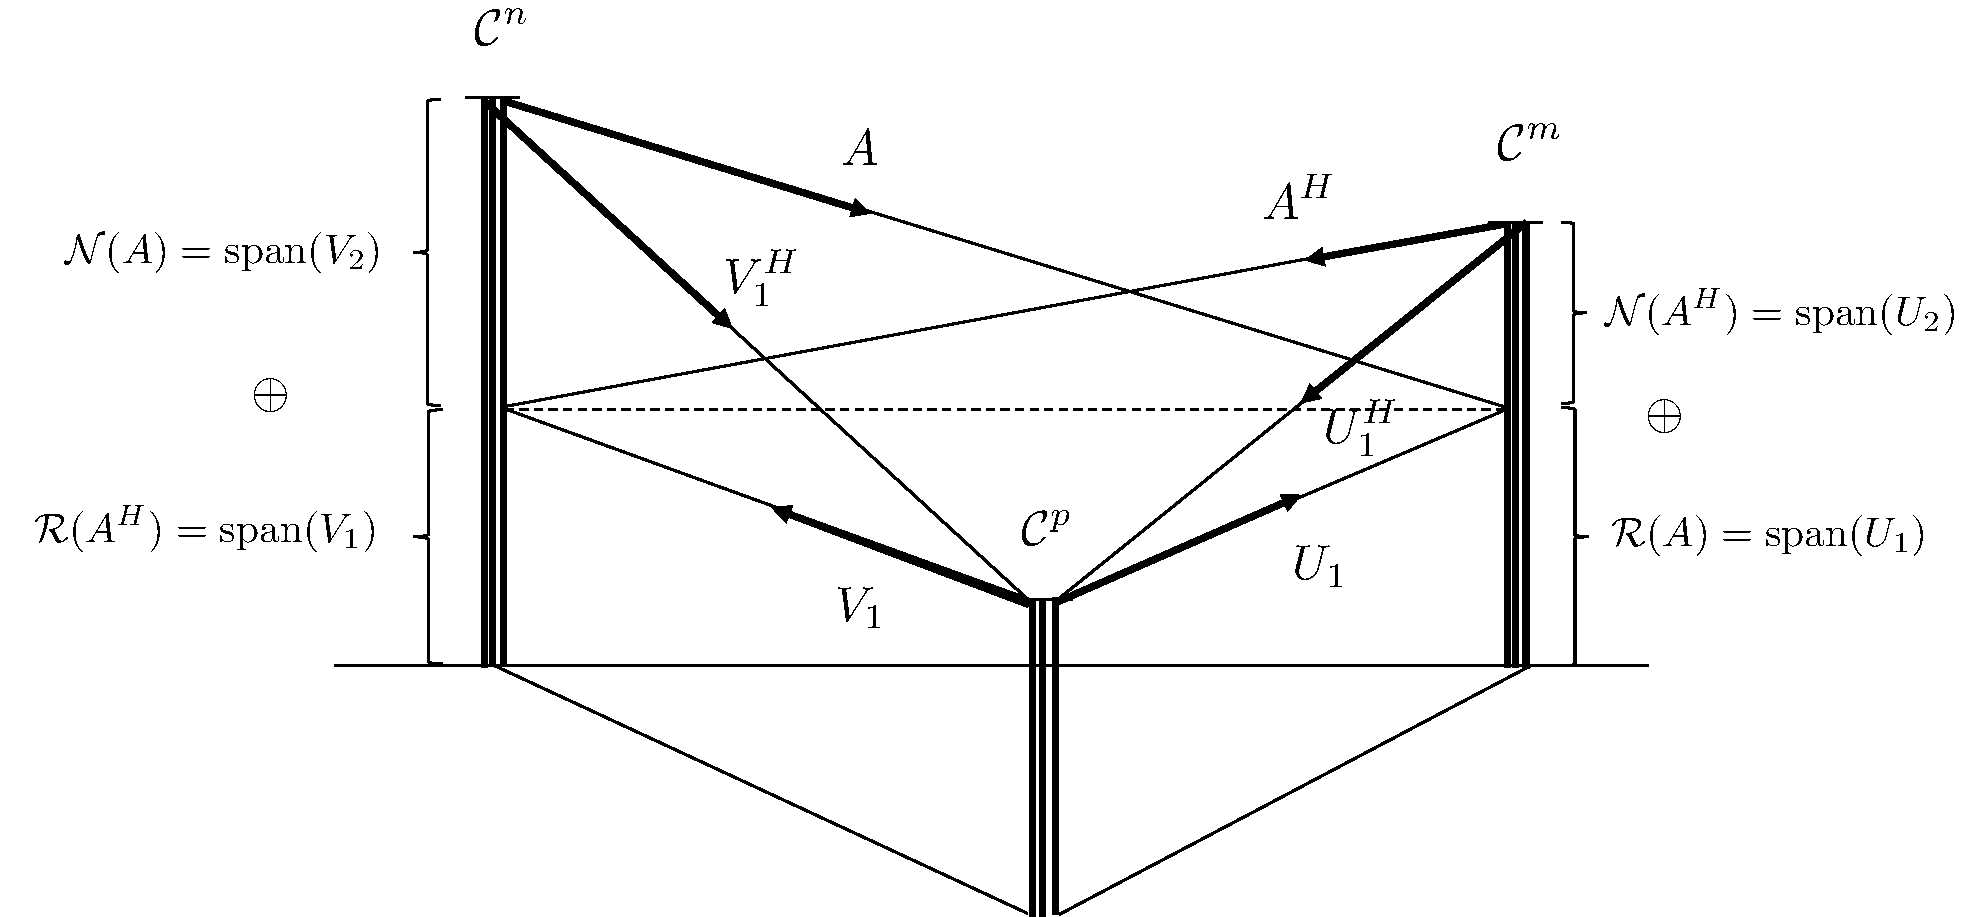
\includegraphics[width=0.9\textwidth]
			{figures/chap7_svd_1}
	\end{center}	
	Since $rank(A) = p$ we can only take inverses in 
	$\mathbb{C}^p$.  
	Therefore instead of solving $Ax=b$ directly in 
	$\mathbb{C}^n$ and 
	$\mathbb{C}^m$ we go indirectly through $\mathbb{C}^p$.
\end{frame}

%----------------------------------
\begin{frame}\frametitle{SVD and Pseudo Inverse: Not Full Rank $A$}
	\par\noindent{\color{blue}Step 1: Least Squares}
	
	Recall that to solve $\min\norm{Ax-b}_2$ when $A$ is full rank:
	\begin{center}
		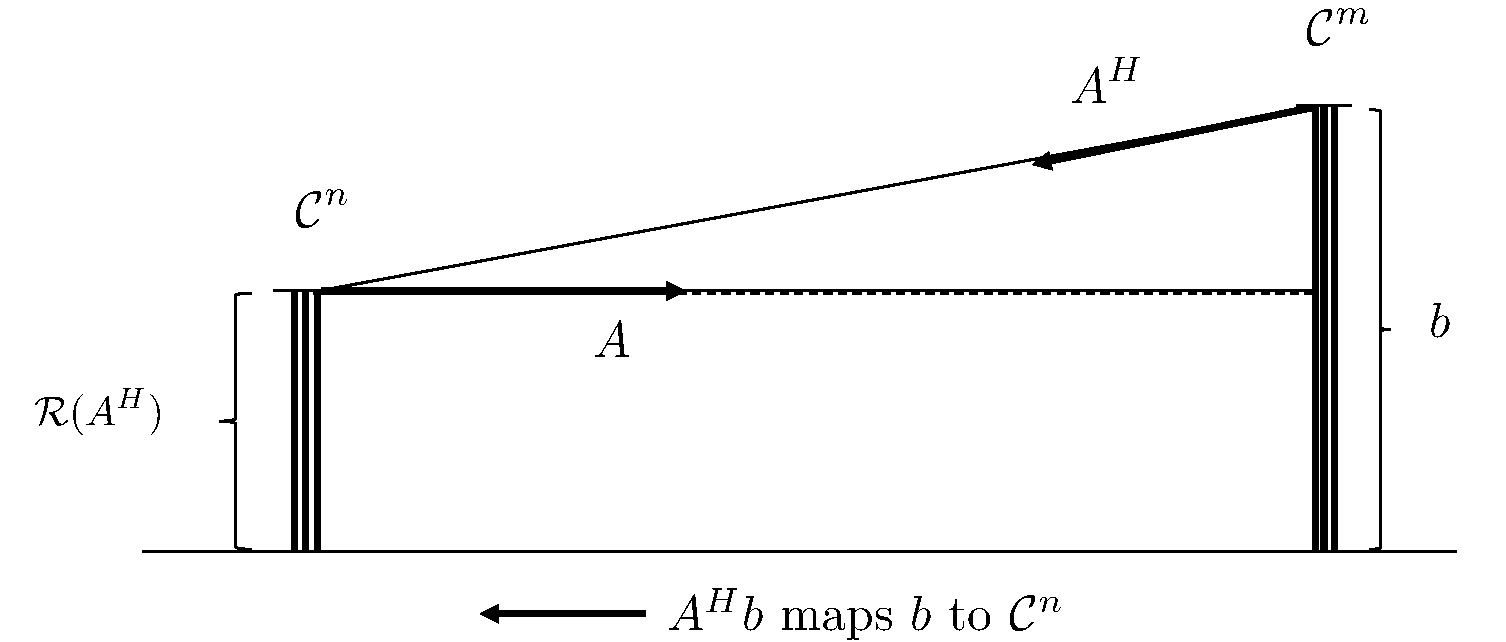
\includegraphics[width=0.9\textwidth]
			{figures/chap7_svd_2}
	\end{center}
	where we can invert things, i.e.
	\begin{align*}
		& A^HAx = A^Hb \\
		\implies & \hat{x} = (A^H A)^{-1} A^H b.
	\end{align*}
\end{frame}

%----------------------------------
\begin{frame}\frametitle{SVD and Pseudo Inverse: Not Full Rank $A$}
	So we have the following:
	\begin{center}
		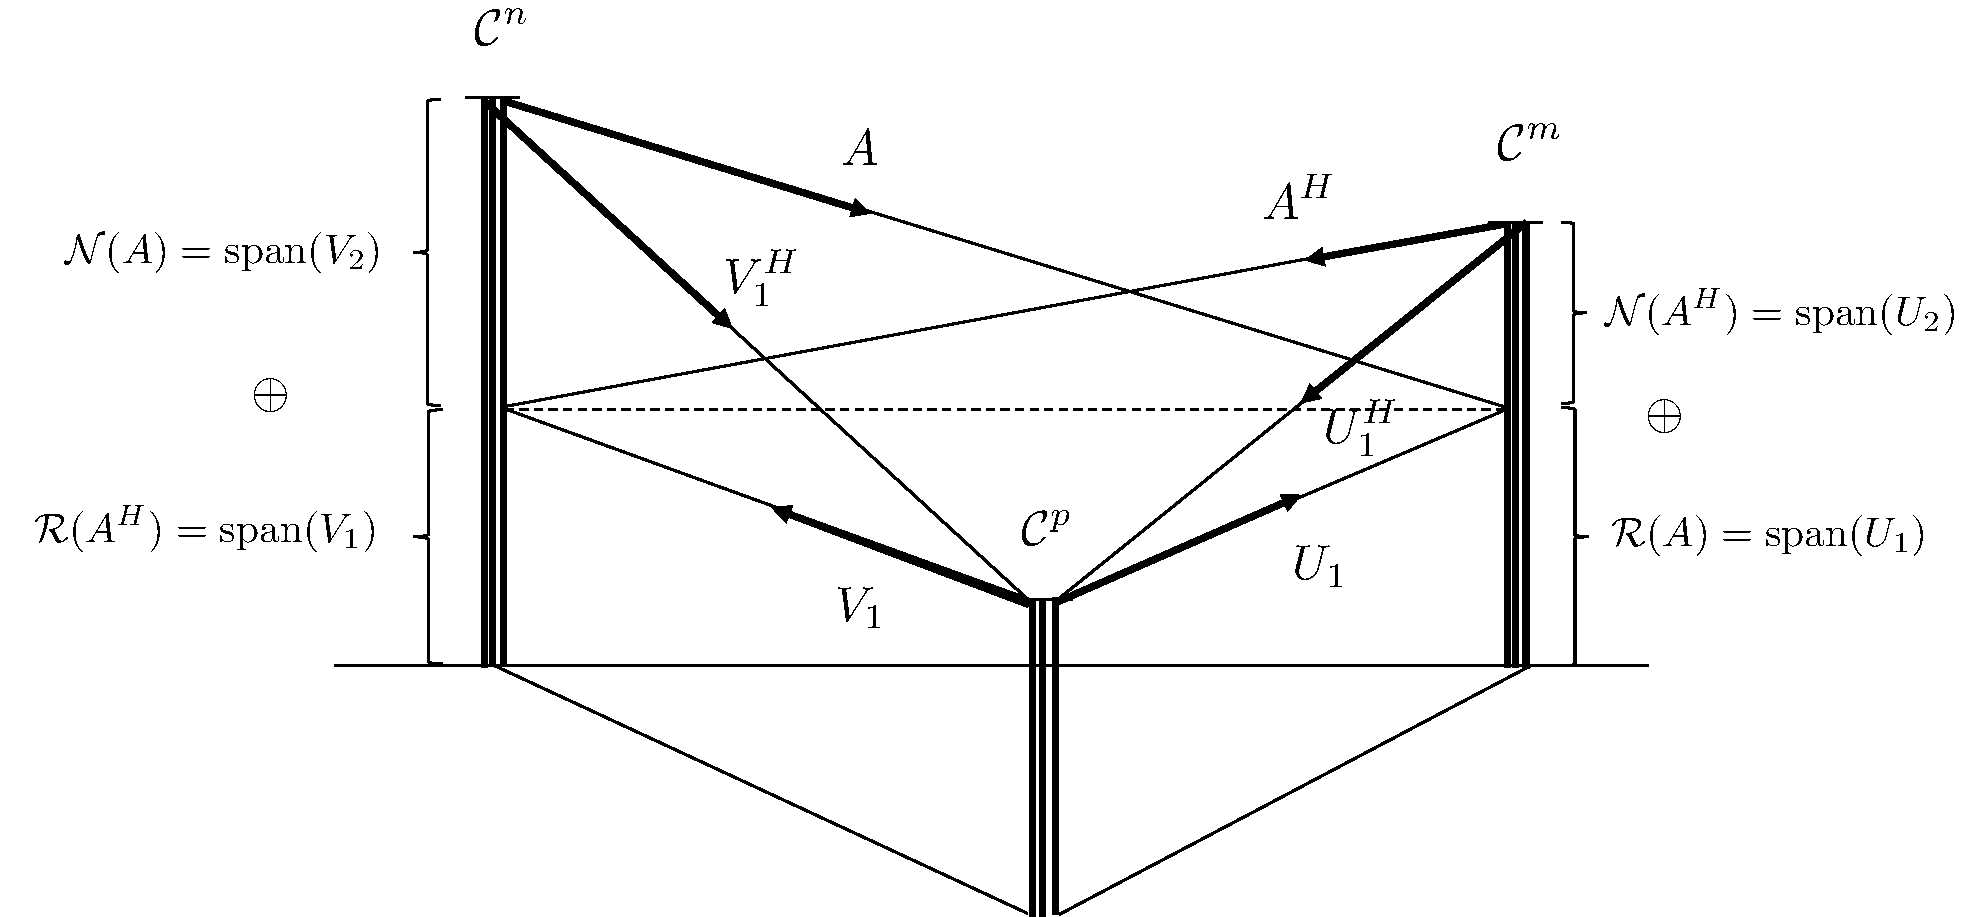
\includegraphics[width=0.9\textwidth]
			{figures/chap7_svd_1}
	\end{center}
	Now instead of $A^H$ we use $U_1^H$ to map to $\mathbb{C}^p$, i.e., given
	\[ 
		Ax = b
	\]
	map to $\mathbb{C}^p$ using $U_1^H$ to get:
	\[
		U_1^HAx = U_1^Hb \qquad \in\mathbb{C}^p.
	\]	
\end{frame}

%----------------------------------
\begin{frame}\frametitle{SVD and Pseudo Inverse: Not Full Rank $A$}
	\par\noindent{\color{blue}Step 2: Minimum Norm}
	
	Recall that to $\min\norm{x}$ such that $Ax = b$, $A$-full rank,
	\begin{center}
		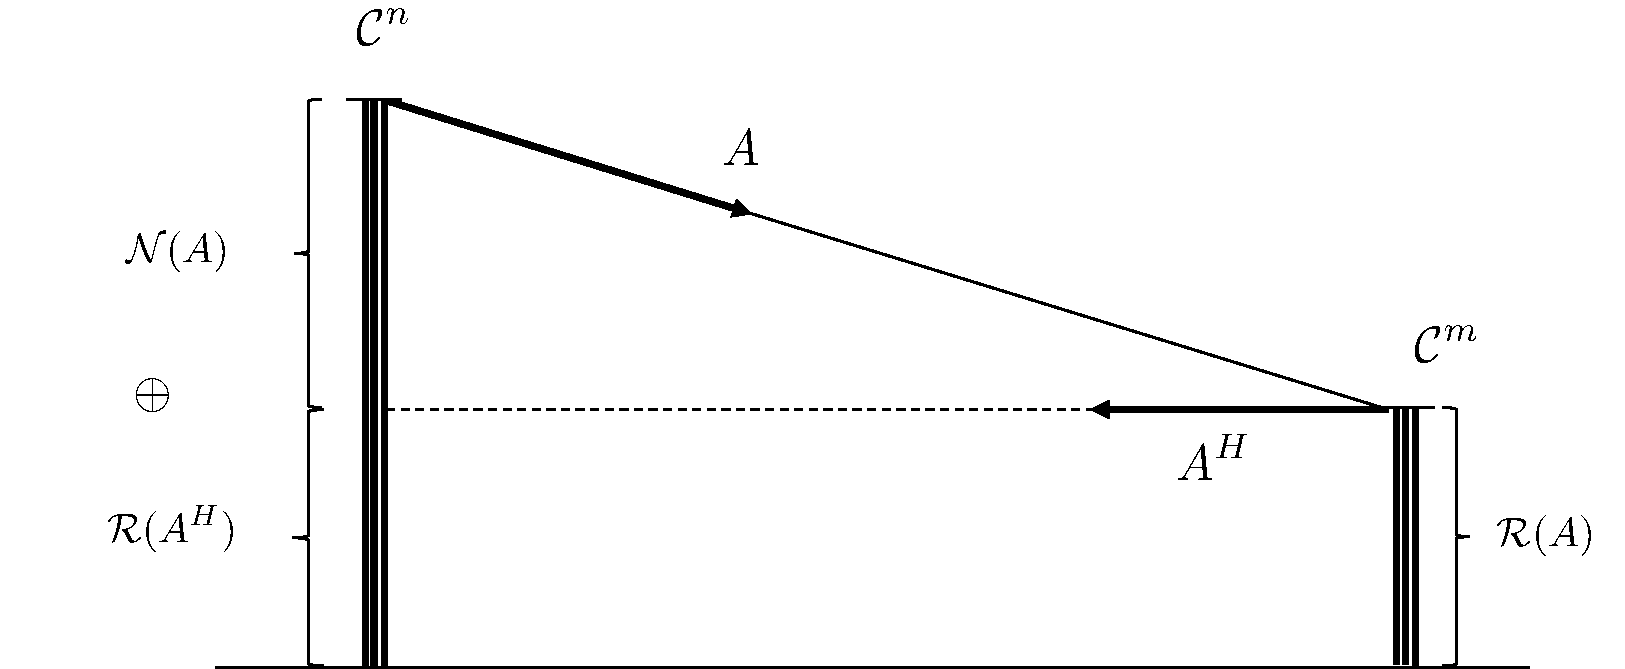
\includegraphics[width=0.7\textwidth]
			{figures/chap7_svd_3}
	\end{center}
	to minimize $\norm{x}$ we zero out the part that is in the null space of $A$, i.e. let
	\[ 
		x = A^Hz \text{ where } z \in \mathbb{C}^m 
	\]
	then
	\[ 
		AA^Hz = b 
		\qquad \Rightarrow \qquad 
		z = (AA^H)^{-1}b 
	\]
	so that
	\[ 
		\hat{x} = A^H(AA^H)^{-1}b.
	\]
\end{frame}

%----------------------------------
\begin{frame}\frametitle{SVD and Pseudo Inverse: Not Full Rank $A$}
	\begin{columns}
		\begin{column}{0.5\textwidth}
			In our case, again pick $x$ to zero the portion in the null space of $A$.  Let
			\[ 
				x = V_1z \quad \text{ where }  \quad z \in \mathbb{C}^p 
			\] 
			so that 
			\[ 
				U_1^HAx = \left(U_1AV_1\right) z = U_1^Hb. 
			\]	
			Note that 
			\[
				U_1AV_1: \mathbb{C}^p \to \mathbb{C}^p.
			\]
		\end{column}
		\begin{column}{0.5\textwidth}
			In fact,
			\[ 
				U_1^H A V_1 = U_1^H U_1 \Sigma_1 V_1^H V_1 = \Sigma_1.
			\]
			so we have
			\begin{align*}
				& \Sigma_1 z = U_1^Hb \\
				\implies & z = \Sigma_1^{-1}U_1^Hb \\
				\implies & \fbox{ $\hat{x} = V_1\Sigma_1^{-1}U_1^Hb$ }
			\end{align*}
			\begin{center}
				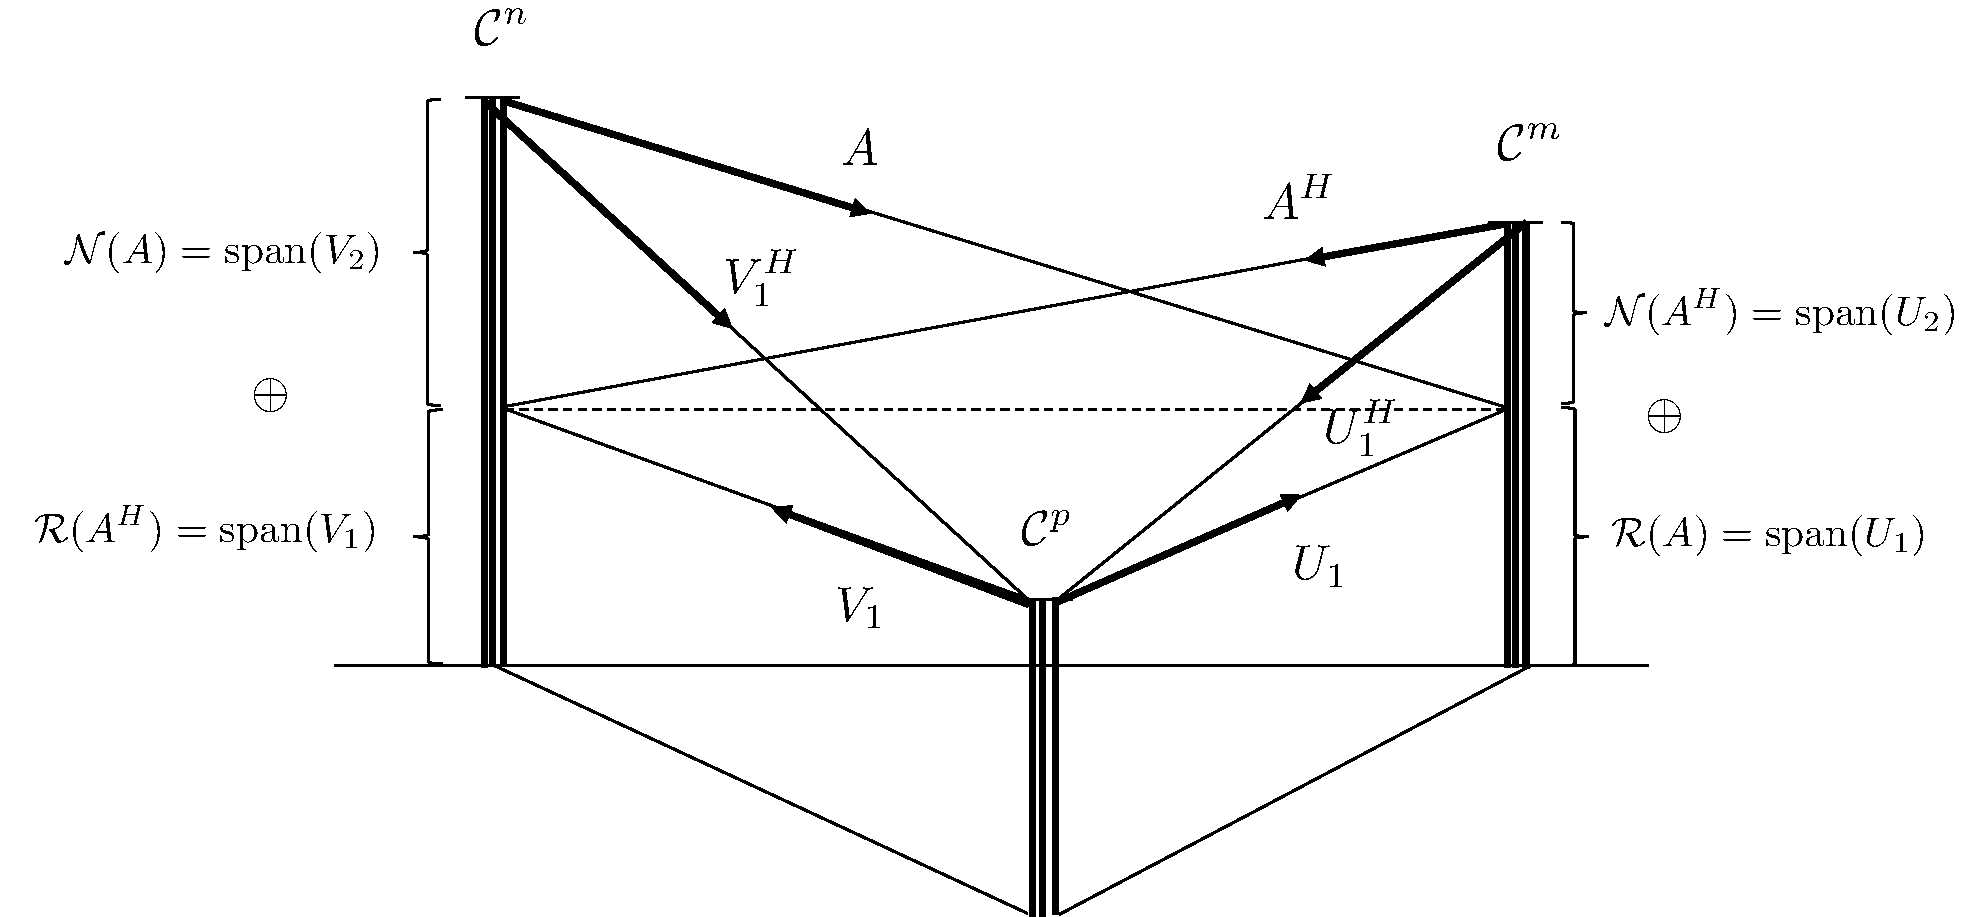
\includegraphics[width=0.9\textwidth]
					{figures/chap7_svd_1}
			\end{center}					
		\end{column}
	\end{columns}


	
\end{frame}


\end{document}